\documentclass[12pt,a4paper]{article}

\usepackage[utf8]{inputenc}
\usepackage[brazilian]{babel}
\usepackage{amsmath}
\usepackage{graphicx}
\usepackage{longtable}
\usepackage{siunitx}
\usepackage{booktabs}
\usepackage{geometry}
\usepackage{float}
\usepackage{indentfirst}
\usepackage{newtxtext}
\usepackage{newtxmath}

\usepackage[authoryear]{natbib}

\geometry{margin=2.5cm}

\title{Determinação da aceleração da gravidade a partir do movimento oscilatório de um pêndulo simples.}
\author{Enzo Rocha Leite Diniz Ribas \\ Centro Federal de Educação Tecnológica de Minas Gerais}
\date{\today}

\begin{document}
\begin{titlepage}

\begin{center}


\includegraphics[width=4cm]{media/Logo_CEFET-MG.png}

\Large
Centro Federal de Educação Tecnológica de Minas Gerais

\vspace{1cm}

\Large
Curso de Engenharia Mecânica

\vspace{2cm}

\Huge
Determinação da aceleração da gravidade a partir do movimento oscilatório de um pêndulo simples.

\vspace{3cm}

\begin{flushright}
\Large
Mecânica, Oscilações, Fluidos e Termodinâmica, Turma T03 \\
Prof. Dr. Mauro Lucio Lobão Iannini
\end{flushright}

\vspace{3cm}

\large
Enzo Rocha Leite Diniz Ribas (Eng. Mecânica - 20253002819)\\
Gabriel Resende Amorim Oliveira (Eng. Elétrica - 20233014438)\\
Leandro Césari e Silva Barros (Eng. Mecânica - 20253005104)\\

\vfill

\Large
Belo Horizonte

\Large
\the\year/{1}

\end{center}

\end{titlepage}

\section{Introdução}

O roteiro do experimento \citep{Roteiro_Experimento_05} propõe a determinação da aceleração da gravidade a partir do movimento oscilatório de um pêndulo simples.

\section{Fundamentação Teórica}

\begin{figure}[H]
\centering
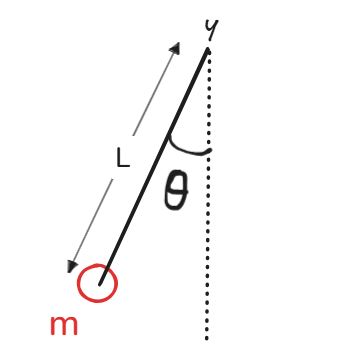
\includegraphics[width=0.8\textwidth]{media/graphs/diagrama}
\caption{Diagrama de um sistema de pêndulo simples. Fonte: Autor}
\label{fig:free_body_diagram}
\end{figure}

Considere uma massa $m$ pendente de um fio de comprimento $L$, formando um ângulo $\theta$ com a vertical. Ao perturbar o sistema, a massa inicia um movimento oscilatório. A força restauradora que atual sobre a massa vem da componente tangencial da força peso:
\begin{equation}
F_{restauradora} = -mg \sin(\theta).
\end{equation}

A expressão equivalente para o torque $\tau$ em relação ao ponto de suspensão é dada por
\begin{equation}
\uptau = -mgL \sin(\theta), \label{eq:torque_pendulum}
\end{equation}

Sabemos da segunda lei de Newton para rotação que o torque é igual ao momento de inércia $I$ multiplicado pela aceleração angular $\alpha$, e que o momento de inércia de uma massa pontual é dado por $I = mL^2$. Assim, podemos escrever a segunda lei de Newton para rotação para o sistema do pêndulo como:
\begin{align*}
    \uptau &= I \alpha \\
    &= m L^2 \alpha \\
    &= m L^2 \frac{d^2\theta}{dt^2}
\end{align*}
Igualando as expressões para o torque da equação \eqref{eq:torque_pendulum} e da segunda lei de Newton para rotação, temos
\begin{align}
    -mgL \sin(\theta) &= m L^2 \frac{d^2\theta}{dt^2} \nonumber \\
    -\frac{g}{L} \sin(\theta) &= \frac{d^2\theta}{dt^2} \nonumber \\
    \frac{d^2\theta}{dt^2} + \frac{g}{L} \sin(\theta) &= 0
    \label{eq:equacao_diferencial_pendulo}
\end{align}
Essa é a equação diferencial não linear que descreve o movimento do pêndulo simples.
A expansão em série de Taylor para função $\sin(\theta)$ em torno de $\theta = 0$ é dada por
\begin{equation}
    \sin(\theta) = \theta - \frac{\theta^3}{3!} + \frac{\theta^5}{5!} - \cdots
    \label{eq:expansao_taylor_sin}
\end{equation}

Substituindo a expansão em série de Taylor da função $\sin(\theta)$ na equação diferencial do pêndulo simples, temos
\begin{align*}
    \frac{d^2\theta}{dt^2} + \frac{g}{L} \left( \theta - \frac{\theta^3}{3!} + \frac{\theta^5}{5!} - \cdots \right) &= 0 \\
    \frac{d^2\theta}{dt^2} + \frac{g}{L} \theta - \frac{g}{L} \frac{\theta^3}{3!} + \frac{g}{L} \frac{\theta^5}{5!} - \cdots &= 0
\end{align*}
Ao truncar a expansão na primeira ordem, o erro introduzido é da ordem de $\theta^3$, o que é pequeno para pequenas oscilações. Portanto, a aproximação $\sin(\theta) \approx \theta$ é válida para pequenas oscilações, e a equação diferencial do pêndulo simples pode ser linearizada para pequenas oscilações resultando na seguinte equação diferencial linear:
\begin{equation}
    \frac{d^2\theta}{dt^2} + \frac{g}{L} \theta = 0, \label{eq:equacao_diferencial_pendulo_linearizada}
\end{equation}

Que é uma equação diferencial de segunda ordem homogênea com coeficientes constantes.
Determinando um polinômio característico para a equação diferencial linearizada, temos
\begin{align}
    \frac{d^2\theta}{dt^2} + \frac{g}{L} \theta &= 0 \nonumber \\
    \left(\frac{d^2}{dt^2} + \frac{g}{L}\right) \theta &= 0
\end{align}
O polinômio característico é dado por
\begin{equation}
    r^2 + \frac{g}{L} = 0,
\end{equation}
Calculando as raízes do polinômio característico, temos
\begin{align*}
    r^2 &= -\frac{g}{L} \\
    \implies \Delta &= 0 - 4 \cdot \frac{g}{L} = -\frac{4g}{L} < 0 \\
    \implies r &= \pm \frac{\sqrt{-\frac{4g}{L}}}{2} = \pm \sqrt{(-1)\frac{4g}{4L}}\\
    &= \pm i \sqrt{\frac{g}{L}} \\
    \therefore r_1 &= i \sqrt{\frac{g}{L}}, \quad r_2 = -i \sqrt{\frac{g}{L}} \\
\end{align*}
Agora podemos reecrever a equação na forma fatorada, utilizando as raízes do polinômio característico, temos
\begin{align*}
    \left(\frac{d^2}{dt^2} + \frac{g}{L}\right) \theta &= 0 \\
    \left(\frac{d}{dt} - r_1\right)\left(\frac{d}{dt} - r_2\right) \theta &= 0 \\
    \left(\frac{d}{dt} - i \sqrt{\frac{g}{L}}\right)\left(\frac{d}{dt} + i \sqrt{\frac{g}{L}}\right) \theta &= 0 \\
\end{align*}
Se o primeiro fator for igual a zero, temos
\begin{align*}
    \left(\frac{d}{dt} - i \sqrt{\frac{g}{L}}\right) \theta &= 0 \\
    \implies \frac{d\theta}{dt} - i \sqrt{\frac{g}{L}} \theta&= 0
\end{align*}
Que é uma equação diferencial de primeira ordem homogênea linear, e a solução geral para essa equação é dada por
\begin{align*}
    \theta(t)_{1} &= C \cdot exp\left(i \sqrt{\frac{g}{L}} t\right) \\
\end{align*}
Se o segundo fator for igual a zero, temos
\begin{align*}
    \left(\frac{d}{dt} + i \sqrt{\frac{g}{L}}\right) \theta &= 0 \\
    \implies \frac{d\theta}{dt} + i \sqrt{\frac{g}{L}} \theta&= 0
\end{align*}
e a solução geral para essa equação é dada por
\begin{align*}
    \theta(t)_{2} &= D\cdot exp\left(-i \sqrt{\frac{g}{L}} t\right) \\
\end{align*}
Pelo teorema de superposição, a combinação linear das soluções $\theta(t)_{1}$ e $\theta(t)_{2}$ é também uma solução para a equação diferencial linearizada do pêndulo simples, e a solução geral para a posição angular do pêndulo simples é dada por
\begin{align*}
    \theta(t) &= C \cdot exp\left(i \sqrt{\frac{g}{L}} t\right) + D \cdot exp\left(-i \sqrt{\frac{g}{L}} t\right)
\end{align*}
Da fórmula compacta de Euler, sabemos que $exp(i \theta) = \cos(\theta) + i \sin(\theta)$, e utilizando essa fórmula, podemos reescrever a solução geral para a posição angular do pêndulo simples como
\begin{align}
    \theta(t) & = C \cdot \left(\cos\left(\sqrt{\frac{g}{L}} t\right) + i \sin\left(\sqrt{\frac{g}{L}} t\right)\right) + D \cdot \left(\cos\left(-\sqrt{\frac{g}{L}} t\right) + i \sin\left(-\sqrt{\frac{g}{L}} t\right)\right) \nonumber \\
    & = C \cdot \left(\cos\left(\sqrt{\frac{g}{L}} t\right) + i \sin\left(\sqrt{\frac{g}{L}} t\right)\right) + D \cdot \left(\cos\left(\sqrt{\frac{g}{L}} t\right) - i \sin\left(\sqrt{\frac{g}{L}} t\right)\right) \nonumber \\
    & = (C + D) \cdot \cos\left(\sqrt{\frac{g}{L}} t\right) + i (C - D) \cdot \sin\left(\sqrt{\frac{g}{L}} t\right) \label{eq:solucao_geral_pendulo}
\end{align}

Pela identidade trigonométrica $\sin(a + b) = \sin(a)\cos(b) + \cos(a)\sin(b)$, queremos reescrever a solução na forma de um único seno com fase:
\begin{equation}
\theta(t) = A\sin\left(\sqrt{\frac{g}{L}} t + \phi\right)~\label{eq:seno_da_fase}
\end{equation}
Fazendo a expansão pela identidade trigonométrica, temos
\begin{align*}
A\sin\left(\sqrt{\frac{g}{L}} t + \phi\right)
&= A\sin\left(\sqrt{\frac{g}{L}} t\right)\cos\phi + A\cos\left(\sqrt{\frac{g}{L}} t\right)\sin\phi
\end{align*}
Igualando termo a termo com a expressão original da equação~\ref{eq:solucao_geral_pendulo}:
\begin{align}
A\sin\phi &= (C + D) \nonumber \\
A\cos\phi &= i (C - D) \nonumber \\
\implies \tan\phi &= \frac{C + D}{i (C - D)} \nonumber \\
\implies \phi &= \arctan\left(\frac{C + D}{i (C - D)}\right) \nonumber
\end{align}

Para encontrar A:
\begin{align*}
\left(A\sin\phi \right)^2 &= \left( { C + D } \right)^2 \\ 
\left(A\cos\phi \right)^2 &= \left( { i^2 C - D} \right)^2 \\
\implies A^2 &= \left( {C + D} \right)^2 + i^2 \left( {C - D} \right)^2 \\
A &= \sqrt{\left( {C + D} \right)^2 - \left( {C - D} \right)^2} \\
&= \sqrt{4CD} = 2 \sqrt{CD}
\end{align*}

Substituindo os valores de $A$ e $\phi$ na equação \eqref{eq:seno_da_fase}, temos a solução geral para a posição angular do pêndulo simples na forma de um único seno com fase:
\begin{align*}
\theta(t) = 2 \sqrt{CD} \sin\left(\sqrt{\frac{g}{L}} t + \arctan\left(\frac{C + D}{i (C - D)}\right)\right)
\end{align*}
em que $A = 2 \sqrt{CD}$ é a amplitude da oscilação, e $\phi = \arctan\left(\frac{C + D}{i (C - D)}\right)$ é a fase inicial. A frequência angular $\omega$ do movimento oscilatório é dada por $\omega = \sqrt{\frac{g}{L}}$

Apesar de conseguirmos chegar a uma expressão para a posição angular, as constantes $C$ e $D$ ainda não foram determinadas, e para isso precisamos de condições iniciais.

Mas para determinar o módulo da aceleração da gravidade $g$, não é necessário determinar as constantes $C$ e $D$, pois basta encontrar uma expressão para o período de oscilação $T$ do pêndulo simples, e a partir disso, determinar $g$ a partir da relação entre o período de oscilação e a frequência angular.

Para determinar uma expressão para o período de oscilação do pêndulo simples, queremos um período $T$ tal que $\theta(t + T) = \theta(t)$ para todo $t$. Substituindo a equação do seno da fase temos
\begin{align*}
\theta(t + T) = A\sin\left(\sqrt{\frac{g}{L}} (t + T) + \phi\right) = A\sin\left(\sqrt{\frac{g}{L}} (t) + \phi\right)
\end{align*}

Utilizando a propriedade do seno:
\begin{align*}
\sin\left(\sqrt{\frac{g}{L}} T + 2\pi\right) &= \sin\left(\sqrt{\frac{g}{L}} T\right) \\
\sqrt{\frac{g}{L}} T &= 2\pi \\
T &= 2\pi \sqrt{\frac{L}{g}} \label{eq:periodo_pendulo}
\end{align*}
No experimento, os dados coletados foram o período de oscilação $T$ para diferentes comprimentos do fio $L$. Para determinar a aceleração da gravidade $g$, podemos rearranjar a equação \eqref{eq:periodo_pendulo} para isolar $g$:

\begin{align*}
T &= 2\pi \sqrt{\frac{L}{g}} \\
\sqrt{\frac{L}{g}} &= \frac{T}{2\pi} \\
\frac{L}{g} &= \left(\frac{T}{2\pi}\right)^2 \\
g &= \frac{L}{\left(\frac{T}{2\pi}\right)^2} \\
&= \frac{4\pi^2 L}{T^2}
\end{align*}

\section{Metodologia}

O experimento foi realizado utilizando um sistema de pêndulo simples, composto por uma massa $m$ pendente de um fio de comprimento $L$. O sistema foi configurado para a contagem do período de oscilação do pêndulo para pequenos ângulos de oscilação.

\begin{figure}[H]
\centering
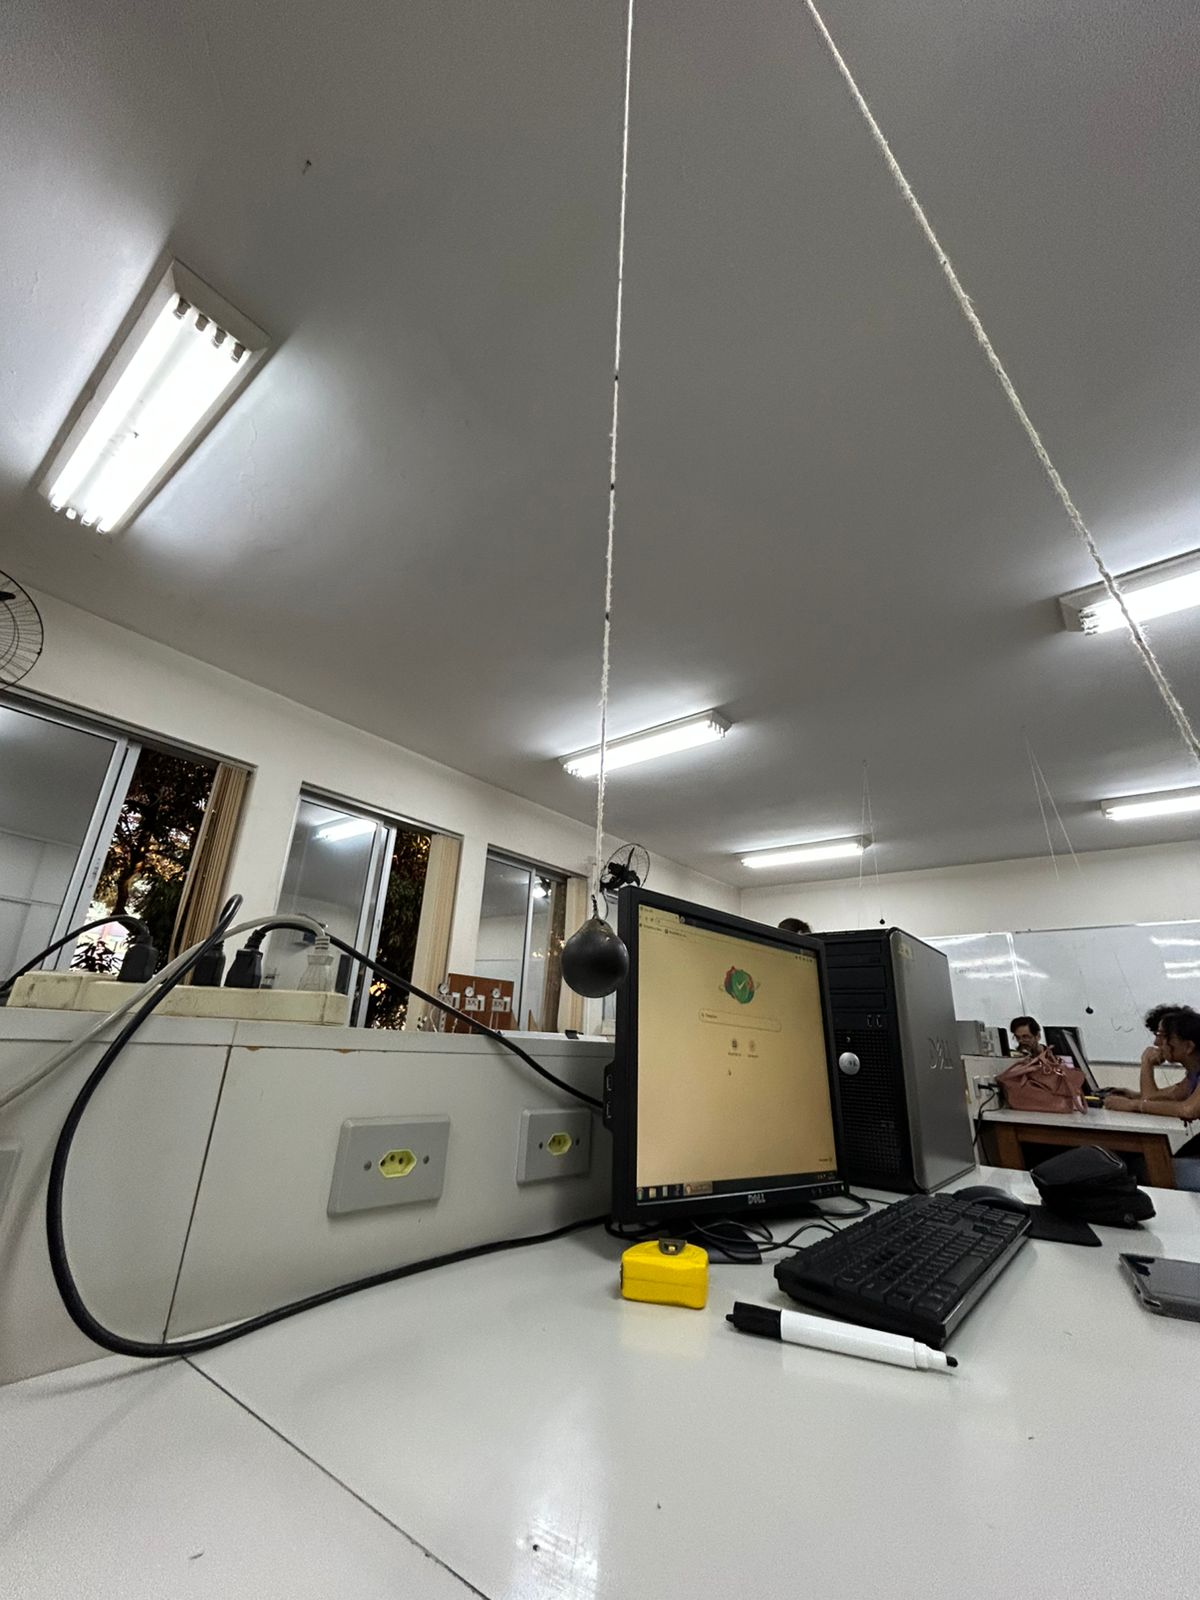
\includegraphics[width=0.8\textwidth]{media/photos/pendulo.png}
\caption{Sistema de pêndulo simples. Fonte: Autor}
\label{fig:pendulo_experimento}
\end{figure}

\begin{figure}[H]
\centering
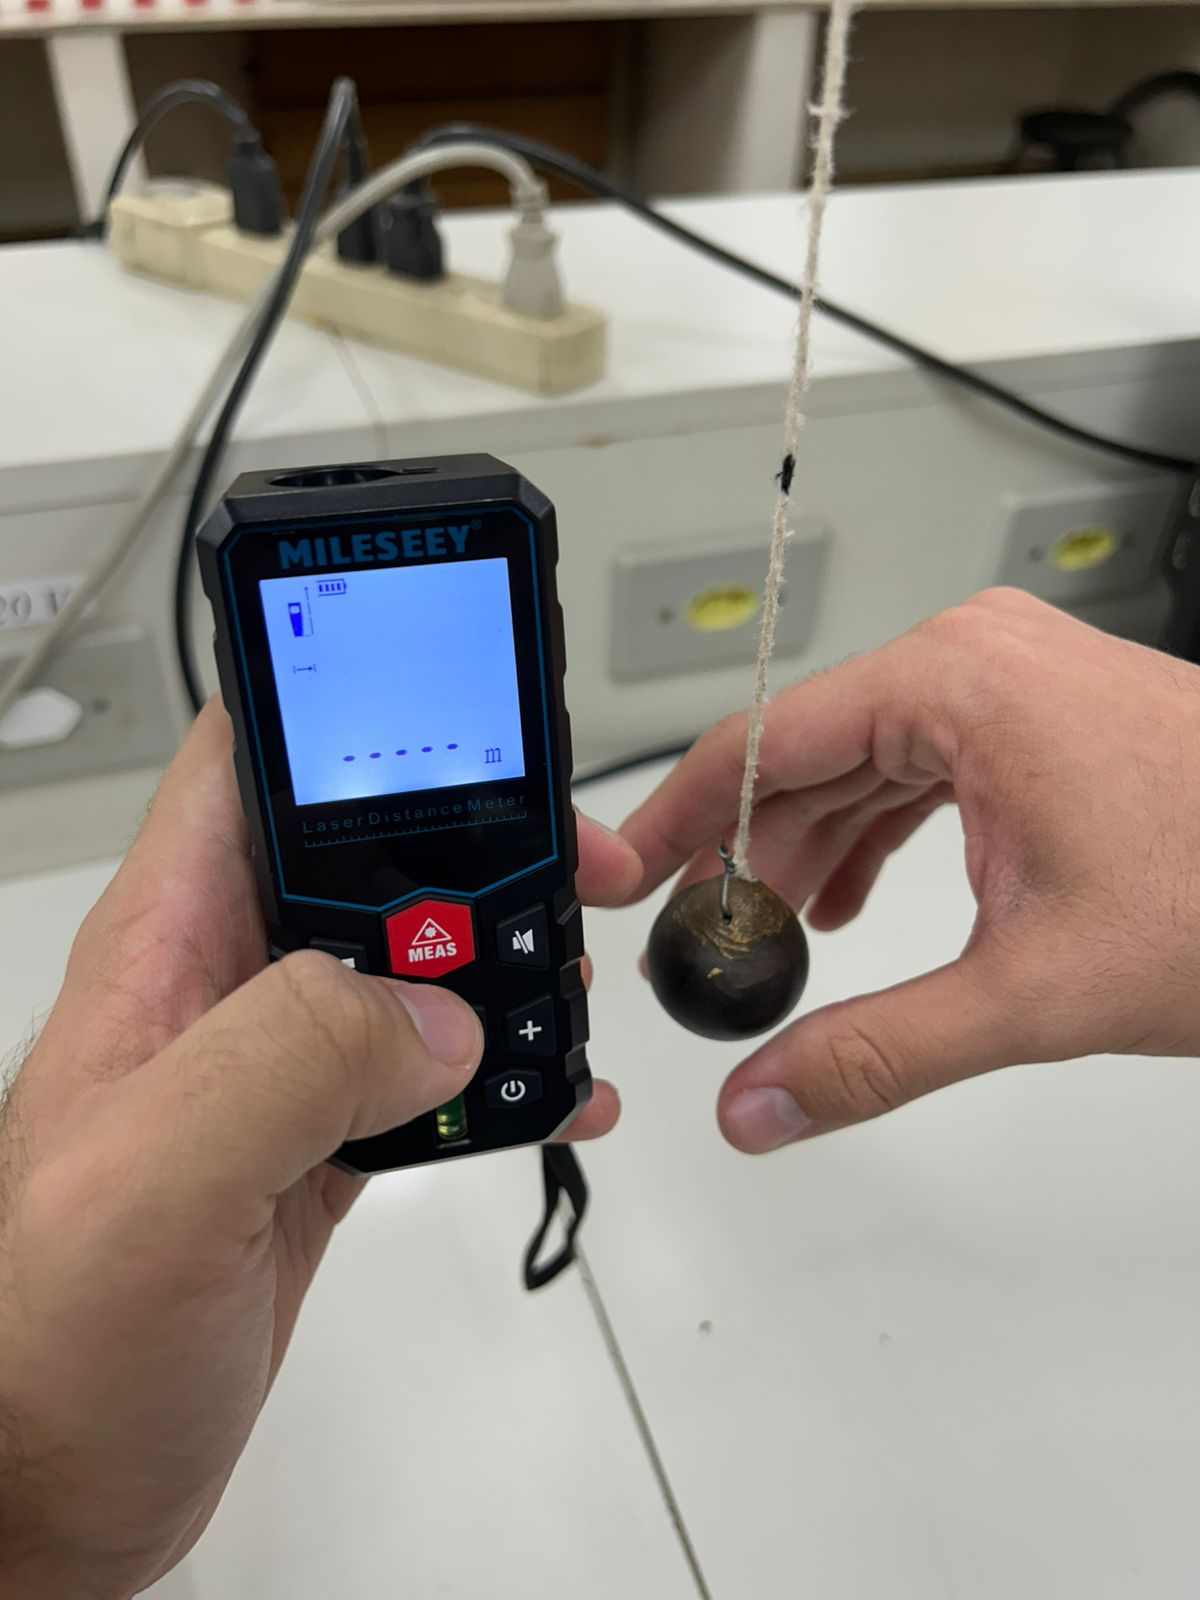
\includegraphics[width=0.8\textwidth]{media/photos/trena_digital.png}
\caption{Trena digital. Fonte: Autor}
\label{fig:trena_digital}
\end{figure}

Os dados do experimento foram anotados em uma tabela para cada comprimento do fio, e posteriormente, a partir dos dados coletados, foi possível determinar a aceleração da gravidade $g$ utilizando o software SciDAVis para análise dos dados e construção de gráficos a partir da linearização dos dados coletados.

\section{Procedimentos}

O procedimento experimental seguiu as seguintes etapas:

\subsubsection{Cronometragem do período de oscilação do pêndulo}
O sistema foi configurado para que a massa pendente pudesse oscilar livremente, e em diversas alturas. Para cada configuração, o tempo de 10 oscilações completas foi cronometrado utilizando um cronômetro digital, e o período de oscilação $T$ foi calculado dividindo o tempo total por 10. Esse processo foi repetido para diferentes comprimentos do fio $L$, e os dados foram anotados em uma tabela para posterior análise.

\subsubsection{Determinação do comprimento do fio}
O comprimento do fio $L$ foi medido utilizando uma trena digital, desde o ponto de suspensão até o centro de massa da massa pendente. Essa medida foi realizada para cada configuração do experimento, e os dados foram anotados em uma tabela para posterior análise.

\subsubsection{Organização dos dados em tabela}
Os dados foram anotados manualmente durante o experimento, e posteriormente organizados em uma tabela para facilitar a análise dos dados. A tabela incluiu as seguintes colunas: comprimento do fio $L$, tempo total para 10 oscilações, período de oscilação $T$.

\subsubsection{Construção de gráficos e realização de ajustes no SciDAVis}
Os dados organizados em tabela foram importados para o software SciDAVis para análise de dados.

Utilizando a linearização da equação \eqref{eq:periodo_pendulo}, foi possível construir um gráfico de $L$ em função de $T^2$, e realizar um ajuste linear para determinar a inclinação da reta, que é dada por $\frac{g}{4\pi^2}$. A partir da inclinação da reta, foi possível determinar a aceleração da gravidade $g$ utilizando a relação:
\begin{align*}
L = \frac{g}{4\pi^2} T^2 + b
\end{align*}

Foram plotados dois gráficos, um considerando a constante de ajuste $b$ como um parâmetro a ser determinado, e outro considerando a constante de ajuste $b$ igual a zero, para comparar os resultados obtidos com os dois modelos de ajuste linear.

A partir dos coeficientes dos ajustes lineares calculados experimentalmente, 
foi possível determinar o módulo da aceleração da gravidade $g$.

\section{Apresentação dos Resultados}

\subsection{Dados Coletados}
Os dados coletados no experimento do pêndulo estão organizados na Tabela~\ref{tab:dados}, que apresenta os valores do comprimento do fio $L$ e o período de oscilação $T$ para cada configuração do experimento.

\begin{table}[H]
\centering
\begin{tabular}{S[table-format=1.3] S[table-format=1.3]}
\toprule
\multicolumn{1}{c}{\shortstack{\textbf{Comprimento do fio} \\ \textbf{$L$ (m)}}} & \multicolumn{1}{c}{\shortstack{\textbf{Período de oscilação} \\ \textbf{$T$ (s)}}} \\
\midrule
2,714 & 1,9 \\
2,507 & 1,648 \\
2,338 & 1,338 \\
2,21 & 1,177 \\
2,046 & 1,036 \\
1,912 & 0,877 \\
1,603 & 0,613 \\
\bottomrule
\end{tabular}
\caption{Dados coletados no experimento do pêndulo.}
\label{tab:dados}
\end{table}

\subsection{Análise dos Dados}

\subsubsection{Ajuste Linear com constante de ajuste}
\begin{figure}[H]
\centering
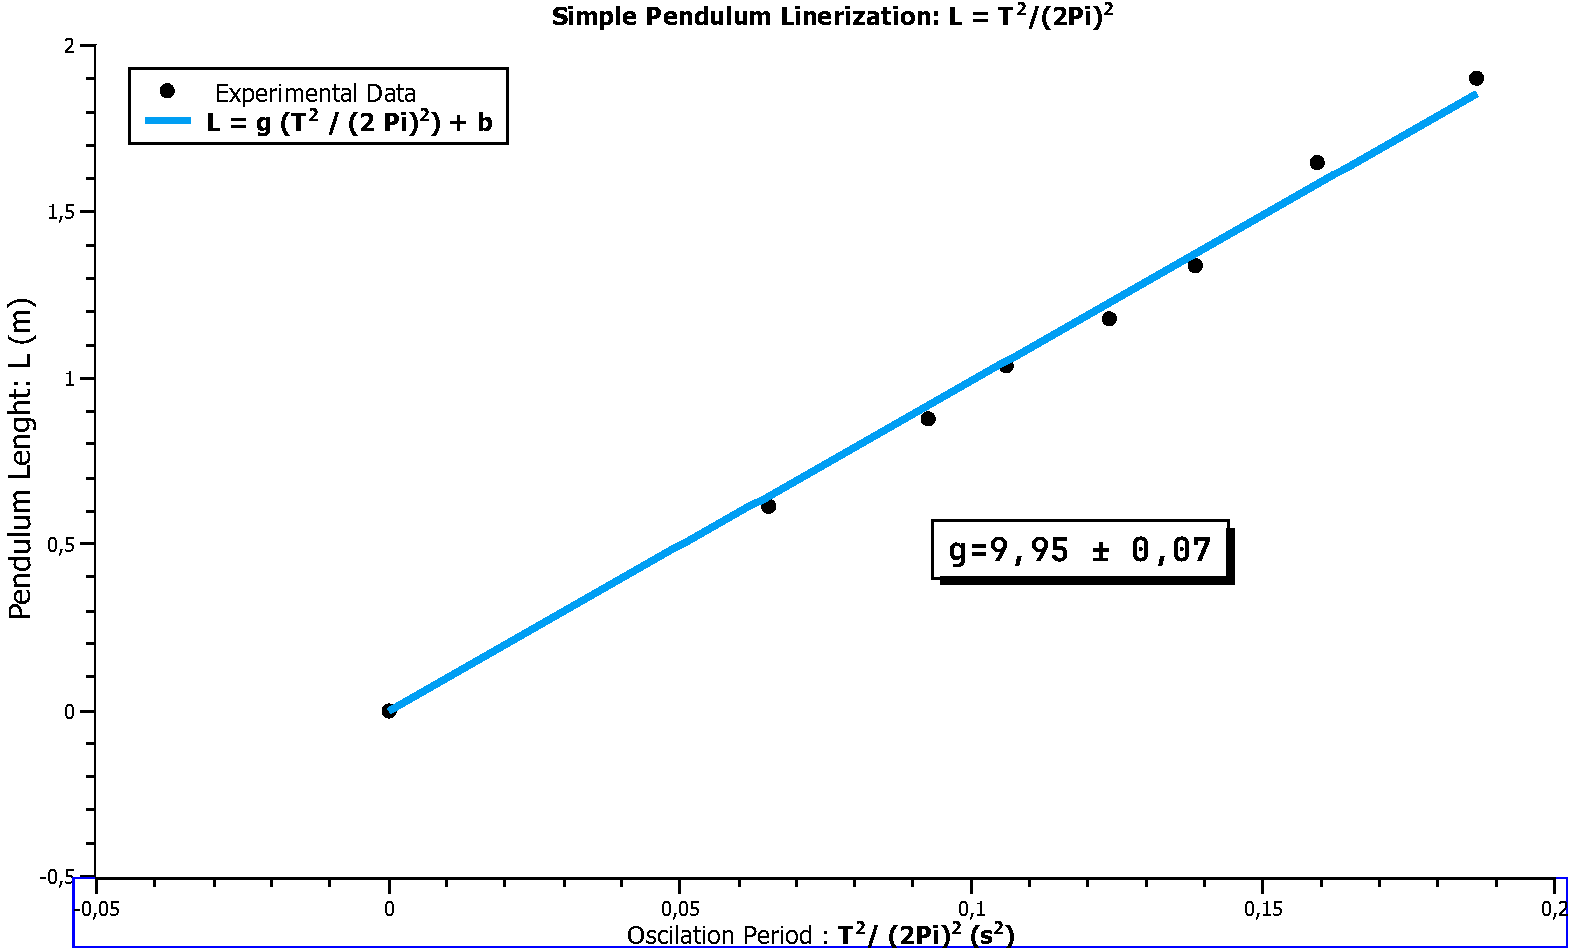
\includegraphics[width=0.8\textwidth]{media/graphs/pendulum_l_2.pdf}
\caption{Ajuste Linear com constante de ajuste. Fonte: Autor}
\label{fig:ajuste_linear_com_constante}
\end{figure}

\subsubsection{Log do SciDAVis}

\begin{verbatim}
[sábado, 25 de abril de 2026 11:25:28 Hora oficial do Brasil	Plot: ''Graph2'']
Non-linear fit of dataset: Table1_l, using function: a*x+b
Y standard errors: Unknown
Scaled Levenberg-Marquardt algorithm with tolerance = 0,0001
From x = 0 to x = 0,186577792296999
a  = 9,95209039767433 +/- 0,0725741275922127
b  = -0,00286887082110515 +/- 0,00456484662317083
--------------------------------------------------------------------------------------
Chi^2 = 0,0137685420208305
R^2 = 0,998825176745932
---------------------------------------------------------------------------------------
Iterations = 1
Status = success
---------------------------------------------------------------------------------------
\end{verbatim}

Valor encontrado de g a partir do ajuste linear com a constante de ajuste: $g = 9,95 \pm 0,07 \, m/s^2$ e constante de ajuste $b = -0,002 \pm 0,004$.

\subsubsection{Ajuste Linear sem constante de ajuste}
\begin{figure}[H]
\centering
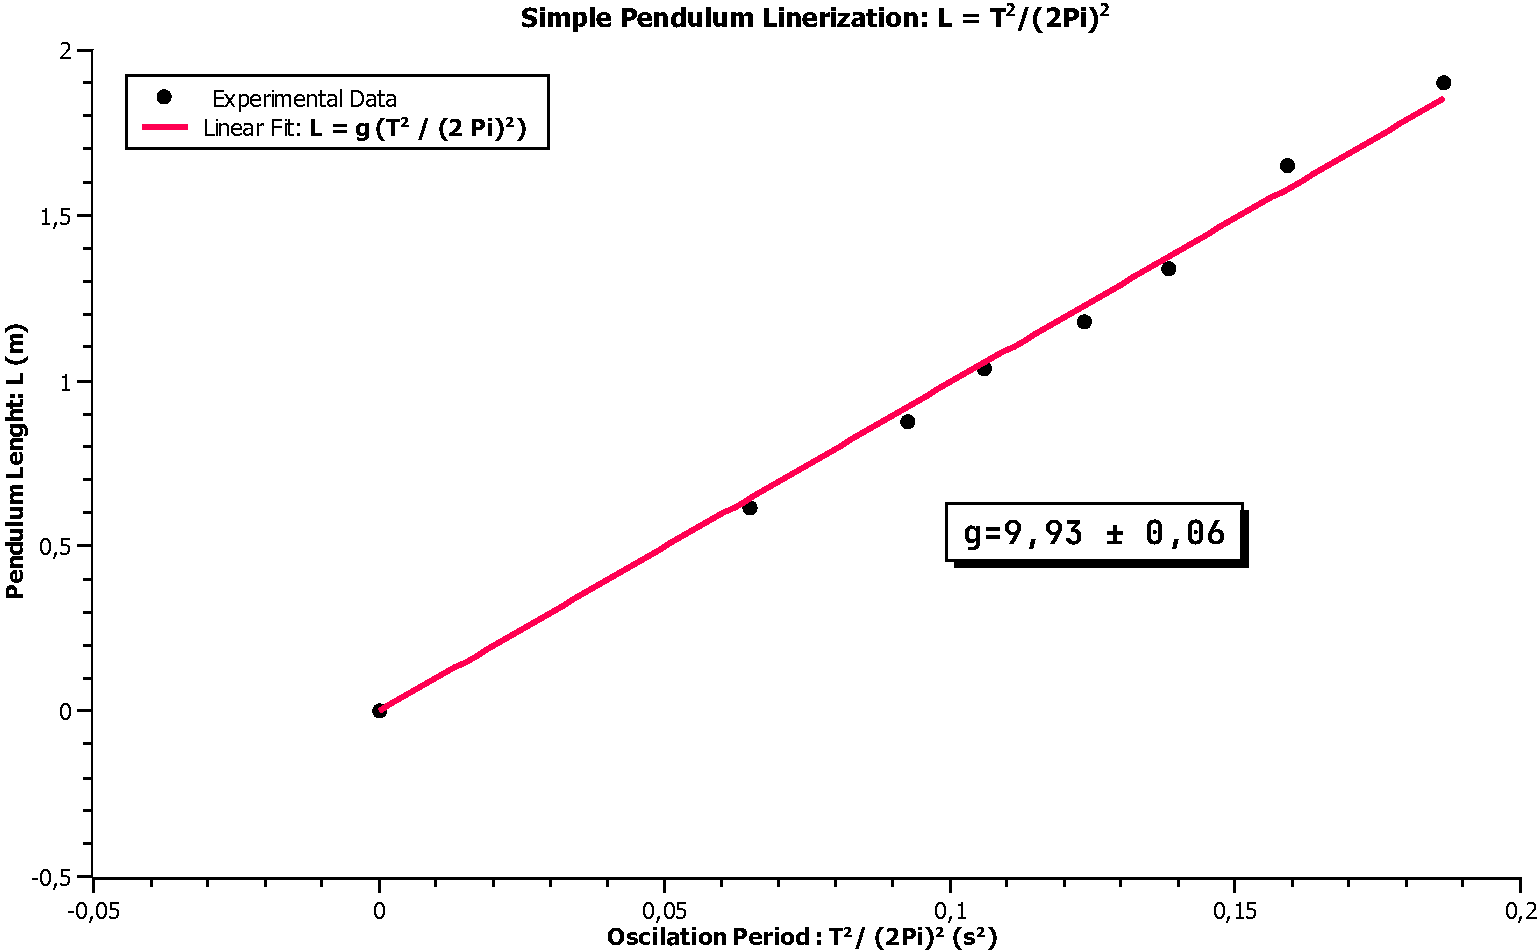
\includegraphics[width=0.8\textwidth]{media/graphs/pendulum_l_1.pdf}
\caption{Ajuste Linear sem constante de ajuste. Fonte: Autor}
\label{fig:ajuste_linear_sem_constante}
\end{figure}
\subsubsection{Log do SciDAVis}
\begin{verbatim}
[sábado, 25 de abril de 2026 11:23:17 Hora oficial do Brasil	Plot: ''Graph1'']
Non-linear fit of dataset: Table1_l, using function: a*x
Y standard errors: Unknown
Scaled Levenberg-Marquardt algorithm with tolerance = 0,0001
From x = 0 to x = 0,186577792296999
a  = 9,93102065416461 +/- 0,0636915352661189
--------------------------------------------------------------------------------------
Chi^2 = 0,0139627645225836
R^2 = 0,998808604394903
---------------------------------------------------------------------------------------
Iterations = 1
Status = success
---------------------------------------------------------------------------------------
\end{verbatim}

Valor encontrado de g a partir do ajuste linear sem constante de ajuste: $g = 9,93 \pm 0,06 \, m/s^2$



\section{Discussão}

Consideramos então, o valor para $g$ encontrado do ajuste sem o termo constante: $g_{exp} = 9,93 \, m/s^2$.

\subsection{Concordância com o Valor de Referência}
Para validar a acurácia experimental, utilizou-se o valor de referência do Observatório Nacional para Belo Horizonte \citep{on_gravimetria_bh_1981}:
\begin{equation}
    g_{bh} = 9{,}7838163 \pm 4\times10^{-7}\,\text{m/s}^2
\end{equation}

O Erro Relativo Percentual ($E_{rel}$) obtido foi de:
\begin{align*}
    E_{rel} &= \frac{|g_{exp} - g_{bh}|}{g_{bh}} \times 100\% \\
\end{align*}
\begin{align*}
\approx \frac{|9,93 - 9,78|}{9,78} \times 100\% \approx 1,53\%
\end{align*}
\section{Conclusão}

O experimento permitiu a determinação da aceleração da gravidade, resultando em $g = 9{,}93 \pm 0{,}06$ m/s$^2$.

A análise dos resultados obtidos a partir dos dois ajustes lineares com e sem constante inicial de ajuste revelou que ambos os modelos forneceram valores para a aceleração da gravidade $g$ que estão próximos do valor esperado de $9,81 \, m/s^2$.

No entanto, o modelo com constante de ajuste apresentou um valor ligeiramente mais alto para $g$, enquanto o modelo sem constante de ajuste apresentou um valor ligeiramente mais baixo. 

A presença da constante de ajuste no modelo pode indicar a existência de um erro sistemático ou uma influência de fatores não considerados no modelo teórico, como a resistência do ar ou a rigidez do fio. 

Por outro lado, o modelo sem constante de ajuste assume que o sistema está idealmente isolado e que todas as condições de contorno são atendidas, o que pode não ser o caso na prática. 

\bibliographystyle{plainnat}
\bibliography{refs}

\end{document}